\documentclass{article}
\usepackage[top=20mm, left=20mm, right=20mm]{geometry}
\usepackage[dvipsnames]{xcolor}
\usepackage{graphicx}
\usepackage{enumerate}
\usepackage{amsmath}
\usepackage{amsfonts}
\usepackage{amsthm}
\usepackage{multicol}
\usepackage{fontspec}
\usepackage{float, graphicx}
\usepackage{cancel}
\usepackage{framed}
\usepackage{tikz}
\usepackage{tkz-euclide}
\usetikzlibrary{automata, positioning, arrows, calc, angles, quotes}
\tikzset{style={font=\scriptsize}}
\usetkzobj{all}
\newcommand{\defLang}[1]{L = \big\{ #1 \big\}}
\newcommand{\derives}{\rightarrow}
\newcommand{\blank}{\textbf{\textvisiblespace}}

\begin{titlepage}
    \title{\textbf{Computer Graphics - Ex. 2}}
    \author{Niv Shani, ID: 311361661}
    \date{}
\end{titlepage}

\begin{document}
    \maketitle
    \vspace{1cm}

    \subsection*{Question 1}
    Prove the following using vector operations only:
    \begin{enumerate}[(a)]
        \begin{framed}
            \item Let $A,B,C\in\mathbb{R}^3$ be the endpoints of a triangle. Let $EF$ be the line segment joining the mid-points of two sides of a triangle. Prove that $EF$ is parallel to the third side ($BC$) and has half of its length.
            \begin{figure}[H]
                \centering
                \includegraphics[width=3.5cm]{q1.png}
            \end{figure}
        \end{framed}
        We'll define the following vector notations:
        $$v = AB\qquad u = AC$$
        Therefore using vector addition, we have:
        $$BC = -v + u = u - v$$
        Doing the same for the two halves, we have:
        $$EF = -\frac{1}{2}v + \frac{1}{2}u = \frac{1}{2}(u - v)$$
        Therefore clearly, $EF \parallel BC$ and has half of its length. $\quad\qedsymbol$
        \newpage
        \item (1) $$\boxed{a\times(b\times c) = (a\cdot c)b-(a\cdot b)c}$$
        Vector cross-prodcut is defined only over $\mathbb{R}^3$, therefore let $$a = (a_1, a_2, a_3),\ b=(b_1,b_2,b_3),\ c=(c_1,c_2,c_3)\in\mathbb{R}^3$$
        Following the definition of cross-product, and vectors commutativity and distributivity properties, we have:
        \begin{align*}
            &a\times(b\times c) = a\times\big( b_2c_3 - b_3c_2,\ b_3c_1 - b_1c_3,\ b_1c_2 - b_2c_1 \big)\\
                &= \begin{bmatrix}
                    a_2\cdot(b_1c_2 - c_1b_2) - a_3\cdot(b_3c_1 - b_1c_3)\\
                    a_3\cdot(b_2c_3 - c_2b_3) - a_1\cdot(b_1c_2 - c_1b_2)\\
                    a_1\cdot(b_3c_1 - b_1c_3) - a_2\cdot(b_2c_3 - c_2b_3)
                \end{bmatrix} =
                \begin{bmatrix}
                    a_2b_1c_2-a_2c_1b_2 - a_3b_3c_1 +a_3b_1c_3\\
                    a_3b_2c_3 - a_3c_2b_3 -a_1b_1c_2 +a_1c_1b_2)\\
                    a_1b_3c_1 - a_1b_1c_3 - a_2b_2c_3 +a_2c_2b_3
                \end{bmatrix}\\
                &= \begin{bmatrix}
                    b_1(a_2c_2 + a_3c_3) -c_1(a_2b_2 + a_3b_3)\\
                    b_2(a_1c_2 + a_3c_3) -c_2(a_1b_1 + a_3b_3)\\
                    b_3(a_1c_1 + a_2c_2) -c_3(a_1b_1 + a_2b_2)
                \end{bmatrix} = \begin{bmatrix}
                    b_1(a_2c_2 + a_3c_3) + a_1b_1c_1-c_1(a_2b_2 + a_3b_3) - a_1b_1c_1\\
                    b_2(a_1c_1 + a_3c_3) +a_2b_2c_2 -c_2(a_1b_1 + a_3b_3) -a_2b_2c_2\\
                    b_3(a_1c_1 + a_2c_2) +a_3b_3c_3 -c_3(a_1b_1 + a_2b_2) -a_3b_3c_3
                \end{bmatrix}\\
                &= \begin{bmatrix}
                    b_1(a_1c_1+a_2c_2 + a_3c_3) -c_1(a_1b_1 + a_2b_2 + a_3b_3)\\
                    b_2(a_1c_1 +a_2c_2+ a_3c_3) -c_2(a_1b_1 +a_2b_2+a_3b_3)\\
                    b_3(a_1c_1 + a_2c_2+a_3c_3) -c_3(a_1b_1 + a_2b_2+a_3b_3)
                \end{bmatrix} = \begin{bmatrix}
                    b_1(a_1c_1+a_2c_2 + a_3c_3)\\
                    b_2(a_1c_1 +a_2c_2+ a_3c_3)\\
                    b_3(a_1c_1 + a_2c_2+a_3c_3)
                \end{bmatrix} - \begin{bmatrix}
                    c_1(a_1b_1 + a_2b_2 + a_3b_3)\\
                    c_2(a_1b_1 +a_2b_2 + a_3b_3)\\
                    c_3(a_1b_1 + a_2b_2+a_3b_3)
                \end{bmatrix}\\
                &= \begin{bmatrix}
                    b_1(a\cdot c)\\
                    b_2(a\cdot c)\\
                    b_3(a\cdot c)
                \end{bmatrix} - \begin{bmatrix}
                    c_1(a\cdot b)\\
                    c_2(a\cdot b)\\
                    c_3(a\cdot b)
                \end{bmatrix} = (a\cdot c)\begin{bmatrix}
                    b_1\\b_2\\b_3
                \end{bmatrix} - (a\cdot b)\begin{bmatrix}
                    c_1\\c_2\\c_3
                \end{bmatrix} = (a\cdot c)b - (a\cdot b)c \quad\qedsymbol
        \end{align*}\\\\
        (2)
        $$\boxed{(a\times b)\times c = (c\cdot a)b-(c\cdot b)a}$$
        \begin{align*}
            &(a\times b)\times c = \big( a_2b_3 - a_3b_2,\ a_3b_1 - a_1b_3,\ a_1b_2 - a_2b_1\big)\times c\\
            &= \begin{bmatrix}
                (a_3b_1 - a_1b_3)\cdot c_3 - (a_1b_2 - a_2b_1)\cdot c_2\\
                (a_1b_2 - a_2b_1)\cdot c_1- (a_2b_3 - a_3b_2)\cdot c_3\\
                (a_2b_3 - a_3b_2)\cdot c_2 - (a_3b_1 - a_1b_3)\cdot c_1
            \end{bmatrix} = \begin{bmatrix}
                a_3b_1c_3 - a_1b_3c_3 - a_1b_2c_2 + a_2b_1c_2\\
                a_1b_2c_1 - a_2b_1c_1 - a_2b_3c_3 + a_3b_2c_3\\
                a_2b_3c_2 - a_3b_2c_2 - a_3b_1c_1 + a_1b_3c_1
            \end{bmatrix}\\
            & = \begin{bmatrix}
                (c_2a_2 + c_3a_3)b_1 - (c_2b_2 + c_3b_3)a_1\\
                (c_1a_1 + c_3a_3)b_2 - (c_1b_1 + c_3b_3)a_2\\
                (c_1a_1 + c_2a_2)b_3 - (c_1b_1 + c_2b_2)a_3
            \end{bmatrix} = \begin{bmatrix}
                (c_2a_2 + c_3a_3)b_1 + a_1b_1c_1 - (c_2b_2 + c_3b_3)a_1 - a_1b_1c_1\\
                (c_1a_1 + c_3a_3)b_2 +a_2b_2c_2  - (c_1b_1 + c_3b_3)a_2 - a_2b_2c_2\\
                (c_1a_1 + c_2a_2)b_3 +a_3b_3c_3 - (c_1b_1 + c_2b_2)a_3 - a_3b_3c_3
            \end{bmatrix}\\
            &= \begin{bmatrix}
                (c_1a_1 + c_2a_2 + c_3a_3)b_1 - (c_1b_1 + c_2b_2 + c_3b_3)a_1\\
                (c_1a_1 +c_2a_2+ c_3a_3)b_2 - (c_1b_1 +c_2b_2+ c_3b_3)a_2\\
                (c_1a_1 + c_2a_2+c_3b_3)b_3 - (c_1b_1 + c_2b_2 + c_3b_2)a_3
            \end{bmatrix} = \begin{bmatrix}
                (c_1a_1 + c_2a_2 + c_3a_3)b_1\\
                (c_1a_1 +c_2a_2+ c_3a_3)b_2\\
                (c_1a_1 + c_2a_2+c_3b_3)b_3
            \end{bmatrix} - \begin{bmatrix}
                (c_1b_1 + c_2b_2 + c_3b_3)a_1\\
                (c_1b_1 +c_2b_2+ c_3b_3)a_2\\
                (c_1b_1 + c_2b_2 + c_3b_2)a_3
            \end{bmatrix}\\
            &= \begin{bmatrix}
                (c\cdot a)b_1\\
                (c\cdot a)b_2\\
                (c\cdot a)b_3
            \end{bmatrix} - \begin{bmatrix}
                (c\cdot b)a_1\\
                (c\cdot b)a_2\\
                (c\cdot b)a_3
            \end{bmatrix} = (c\cdot a)\begin{bmatrix}
                b_1\\b_2\\b_3
            \end{bmatrix} - (c\cdot b)\begin{bmatrix}
                a_1\\a_2\\a_3
            \end{bmatrix} = (c\cdot a)b - (c\cdot b)a\quad\qedsymbol
        \end{align*}
    \end{enumerate}

    \newpage
    \subsection*{Question 2}
    \begin{enumerate}[(a)]
        \begin{framed}
            \item Find an equation for the surface $S$ of points that are equidistant (have the same distnace) from the two points $(-4,2,1),\ (2,-4,3)$. Can you describe $S$?
        \end{framed}
        $S$ is a surface in $\mathbb{R}^3$. Since all the points that lies on $S$ must have equal distance from the two given points, $S$ must be \textbf{a plane}.\\\\
        Particularly, the midpoint between the two given points must lie on $S$, and the normal to the plane must pass through it (since this is the minimal distance to each of the points). We can find these:
        $$p_0 = \bigg(\frac{-4+2}{2},\ \frac{2+(-4)}{2},\ \frac{1+3}{2}\bigg) = (-1,-1,2)$$
        $$\vec{n} = (-4,2,1) - (2,-4,3) = (-6,6,-2)$$
        Each point that lies on $S$, $p = (x,y,z)$ must satisfy:
        $$\vec{n}\cdot((x,y,z) - p_0) = 0$$
        Meaning:
        \begin{align*}
            &\vec{n}\cdot(x+1,y+1,z-2) = 0\\
            \Rightarrow\quad&(-6,6,-2)\cdot(x+1,y+1,z-2) = 0\\
            \Rightarrow\quad&-6x-6+6y+6-2z+4 = 0\\
            \Rightarrow\quad&-6x + 6y -2z + 4 = 0\\
            &\boxed{S:\ \ 3x - 3y +z - 2 = 0}
        \end{align*}
        \begin{framed}
            \item Find an equation for the surface $S$ consisting of \textbf{all points $P$} for which the (unsigned) distance of $P$ from the z-axis is twice the (unsigned) distance of $P$ from the xy-plane.
        \end{framed}
        Firstly, the xy-plane is represented by the implicit equation:
        $$z=0$$
        meaning the distance of a point $p_0 = (x,y,z)$ from the xy-plane is:
        $$|z|$$
        Secondly, the distnace of a point $p_1 = (x,y,z)$ from the z-axis is:
        $$|\sqrt{x^2+y^2}|$$
        Therefore we can use the constaint and get:
        \begin{align*}
            &|\sqrt{x^2+y^2}| = 2\cdot|z|\\
            \Rightarrow\quad&x^2+y^2 = 4z^2\\
            &\boxed{S:\ \ x^2+y^2 - 4z^2 = 0}
        \end{align*}
    \end{enumerate}

    \newpage
    \subsection*{Question 3}
    \begin{framed}
        Find the explicit, implicit and parametric representation of the cone with the following properties:
        \begin{itemize}
            \item It is located on the origin.
            \item It opens in the positive direction of the axis (its one-sided).
            \item The opening angle is $\alpha$, counting from the axis.
        \end{itemize}
        \begin{figure}[H]
            \centering
            \includegraphics[width=3.5cm]{q3.png}
        \end{figure}
    \end{framed}
    Let $P=(x,y,z)$ be a point on the surface of the cone. We can look at the triangle created by $P$, it's projection on the xy-plane, denoted $P'$, and the origin. Since the angle between the cone and the z-axis is $\alpha$, this is the angle in the described triangle, as follows:
    \begin{figure}[H]
        \centering
        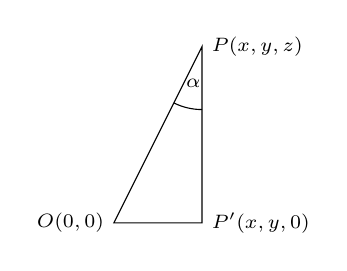
\begin{tikzpicture}[
            scale=2.8,
            my angle/.style={
                every pic quotes/.append,
                draw=black,
                angle radius=.8cm,
            }]
        \coordinate[label=left:{$O(0,0)$}](o) at (0mm,0mm);
        \coordinate[label=right:{$P'(x,y,0)$}](p') at (4mm,0mm);
        \coordinate[label=right:{$P(x,y,z)$}] (p) at (4mm,8mm);
        \draw (p) -- (p') -- (o) -- cycle;
        \pic [my angle, "$\alpha$"] {angle=o--p--p'};
        \end{tikzpicture}
    \end{figure}
    \noindent
    We know that $d\big(P,P'\big) = z$, and $d\big(P',O\big) = \sqrt{x^2+y^2}$. From this we can use $\tan(\alpha)$ to get the implicit representation of the cone:

    $$\tan(\alpha) = \dfrac{\sqrt{x^2+y^2}}{z}\quad\Rightarrow\quad \boxed{x^2+y^2-z^2\tan^2(a) = 0\qquad z\geq 0}$$\\
    \noindent
    We can now solve for $z$ to get the explicit representation:

    $$z^2 = \dfrac{x^2+y^2}{\tan^2(\alpha)}\quad\Rightarrow\quad\boxed{z = \dfrac{\sqrt{x^2+y^2}}{\tan(\alpha)}}$$\\
    For the parametric representation of the cone, we can set $z=t$ as our parameter. Now at each height $t$, we need to construct a circle - remembering the parametric representation of a circle using polar coordinates, we have:
    $$x = t\cos(\alpha)\qquad y=t\sin(\alpha)$$
    Therefore, the parametric representation of the cone is given by:
    $$\boxed{f(x,y,z) = \big(t\cos(\alpha),\ t\sin(\alpha),\ t\big)\qquad t\geq 0}$$

    \newpage
    \subsection*{Question 4}
    \begin{enumerate}[(a)]
        \begin{framed}
            \item Determine if the line given by $f(x,y,z) = (4+3t,-2,1+6t)$, and the plane given by $8x-y+4z=-3$ are parallel, orthogonal or neither.
        \end{framed}
        First, we'll find to points on the given line by plugging $t=0,1$, to find the direction of the line:
        $$p_0 = (4,-2,1)\qquad p_1 = (7,-2,7)$$
        Therefore the direction of the line is given by the vector:
        $$\vec{v} = p_1 - p_0 = (3,0,6)$$
        We can extract the direction of the normal to the given plane, from the given implicit representation coefficients:
        $$\vec{n} = (8,-1,4)$$
        If the line is parallel to the plane, it's direction will be orthogonal to the normal, meaning $\vec{n}\cdot \vec{v} = 0$. However:
        $$\vec{n}\cdot\vec{v} = (8,-1,4)\cdot(3,0,6) = 48 \not= 0$$
        Therefore the line \textbf{is not parallel to the plane}.\\\\
        Similirly, if the line is orthogonal to the plane, then it is parallel to the plane's normal,\\meaning that $\vec{n} = c\vec{v},\ c\in\mathbb{R}$. However, we can see that there'e no such $c$ that satisfies the equation. Therefore, the line \textbf{is not orthogonal to the plane}.\\\\
        Overall, the line is neither parallel nor orthogonal to the plane.$\quad\qedsymbol$
        \vspace{1cm}
        \begin{framed}
            \item Find the intersection of the line $x=12+5t, y=3, z=-4-5t$ and the sphere given by\\$(x-2)^2 + (y-3)^2+(z-1)^2=25$.
        \end{framed}
        Plugging the line parametric representation into the given sphere equation, we have:
        \begin{align*}
            &(12+5t-2)^2 + (3-3)^2 + (-4-5t-1)^2 = 25\\
            &(5t+10)^2 + (-5t-5)^2 = 25\\
            &25t^2+100t+100+25t^2+50t+\cancel{25}=\cancel{25}\\
            &50t^2+150t+100=0\\
            &t^2+3t+2=0\\
            &(t+1)(t+2) = 0\quad\Rightarrow\quad t=-1,-2
        \end{align*}
        Therefore there are two intersection points, and by plugging the values we found for $t$ in the line representation, we have:
        $$\boxed{p_0 = (7,3,1),\ p_1=(2,3,6)}\quad\qedsymbol$$
        \newpage
        \begin{framed}
            \item The points $p_1,p_2$ and $p_3$ are called collinear points if they are located on the same line. Show how to determine if three points are collinear and prove using the proposed condition that the following points $(-1,0,2),\ (1,1,4),\ (3,2,6)$ are collinear.
        \end{framed}
        We can define the vectors:
        $$\vec{v_1} = p_2 - p_1\qquad \vec{v_2} = p_3 - p_2$$

        If $p_1,p_2$ and $p_3$ are located on the same line, the vectors $\vec{v_1},\ \vec{v_2}$ must have the same direction. Meaning, there exists some scalar $c\in\mathbb{R}$, such that $\vec{v_1} = c\vec{v_2}$. If we can find some scalar $c$ that satisfies the condition, we can state that $p_1,p_2$ and $p_3$ are collinear, otherwise they are not.\\\\
        We'll prove using the above proposition with the given points:
        $$p_1=(-1,0,2)\qquad p_2=(1,1,4)\qquad p_3=(3,2,6)$$
        Therefore:
        $$\vec{v_1} = p_2-p_1 = (1,1,4) - (-1,0,2) = (2,1,2)$$
        $$\vec{v_2} = p_3-p_2 = (3,2,6) - (1,1,4) = (2,1,2)$$

        We get that $\vec{v_1} = \vec{v_2}$, and particularly, the condition holds for $c=1$.\\
        Thus, $p_1,\ p_2$ and $p_3$ are collinear.$\quad\qedsymbol$
    \end{enumerate}
\end{document}